% Based on Template from IIS, ETHz
%%%%%%%%%%%%%%%%%%%%%%%%%%%%%%%%%%%%%%%%%%%%%%%%%%%%%%%%%%%%%%%%%%%%%%%
%%%%%%%%%%%%%%%%%%%%%%%%%%%%%%%%%%%%%%%%%%%%%%%%%%%%%%%%%%%%%%%%%%%%%%%
%%%%%                                                                 %
%%%%%     <file_name>.tex                                             %
%%%%%                                                                 %
%%%%% Author:      <author>                                           %
%%%%% Created:     <date>                                             %
%%%%% Description: <description>                                      %
%%%%%                                                                 %
%%%%%%%%%%%%%%%%%%%%%%%%%%%%%%%%%%%%%%%%%%%%%%%%%%%%%%%%%%%%%%%%%%%%%%%
%%%%%%%%%%%%%%%%%%%%%%%%%%%%%%%%%%%%%%%%%%%%%%%%%%%%%%%%%%%%%%%%%%%%%%%

\chapter{Task Description}
Include the task description \textbf{pdf} you got from your
assistant(s) with the \shell{\textbackslash includepdf} command.
% include the task description pdf!
%\includepdf[pages=-, turn=false, scale=0.9]{../../task/TaskDescription.pdf}


\chapter{Declaration of Originality}\label{chap:originality}
Include the declaration of authorship with the \shell{\textbackslash
  includepdf} command (sign it and scan it). For more information
about plagiarism, please visit
\url{https://www.ethz.ch/students/en/studies/performance-assessments/plagiarism.html}

\begin{itemize}
\item \textbf{English version:}
  \url{https://www.ethz.ch/content/dam/ethz/main/education/rechtliches-abschluesse/leistungskontrollen/declaration-originality.pdf}
\item \textbf{German version:}
  \url{https://www.ethz.ch/content/dam/ethz/main/education/rechtliches-abschluesse/leistungskontrollen/plagiat-eigenstaendigkeitserklaerung.pdf}
\end{itemize}

% include the signed declaration of authorship!
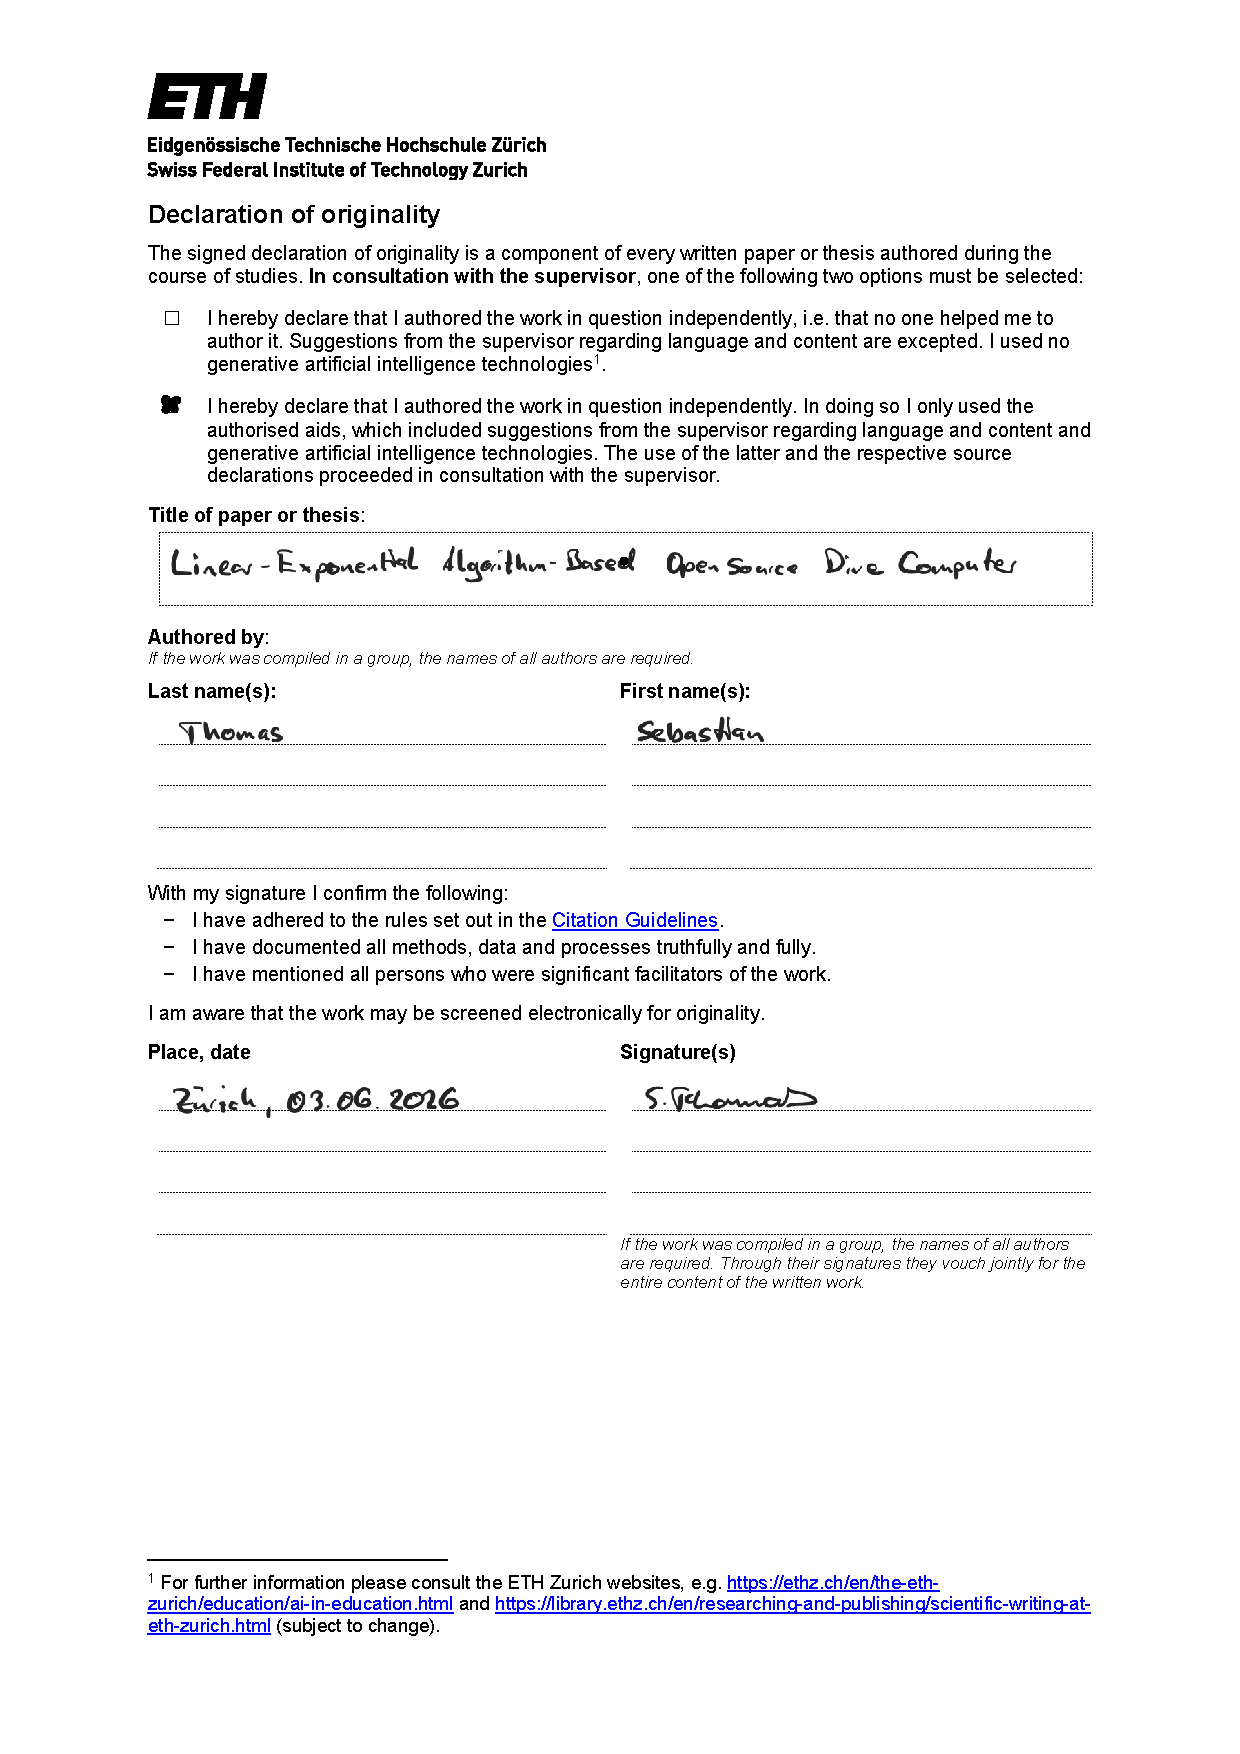
\includepdf[pages=-, turn=false, scale=0.9]{./figures/declaration_of_originality}


\chapter{(optional) File Structure}
Describe how the project directories/files are organized, e.g.:

\begin{flushleft}
\dirtree{%
.1 /.
  .2 README \DTcomment{A README with some general information about the project.}.
  .2 01\_report \DTcomment{The source files of the project report.}.
  .2 02\_presentation \DTcomment{The source files of the presentation.}.
  .2 03\_designflow \DTcomment{Some designflow-specific files.}.
}
\end{flushleft}

What needs to be done to run an RTL simulation (stimuli generation,
compilation...)?


\chapter{(optional) Datasets}
If you have a data set comprising several test images, you could
depict and describe them here. Use a simple naming scheme such that
you can easily refer to certain elements of this data set in the text.


\chapter{(optional) More Evaluation Results}
If you conducted an extensive evaluation you could move surplus
graphs/results to the appendix.